\documentclass[conference]{IEEEtran}
\IEEEoverridecommandlockouts
% The preceding line is only needed to identify funding in the first footnote. If that is unneeded, please comment it out.
\usepackage{cite}
\usepackage{amsmath,amssymb,amsfonts}
\usepackage{algorithmic,algorithm}
\usepackage{graphicx}
\usepackage{textcomp}
\usepackage{xcolor}
\def\BibTeX{{\rm B\kern-.05em{\sc i\kern-.025em b}\kern-.08em
    T\kern-.1667em\lower.7ex\hbox{E}\kern-.125emX}}
\begin{document}

\title{COMP6223 Coursework2: Subverting Face Detection}

\author{\IEEEauthorblockN{Hao Chen}
\IEEEauthorblockA{\textit{Electronics and Computer Science} \\
\textit{University of Southampton}\\
Southampton, United Kingdom \\
hc1u18@soton.ac.uk}
}

\maketitle

\begin{abstract}
This document is the coursework2 report of COMP6223, which the main topic is subverting face detection.
\end{abstract}

\begin{IEEEkeywords}
Haar-Jones Haar Cascade Algorithm, face detection
\end{IEEEkeywords}

% Introduction
\section{Introduction}
This coursework is to explore how to camouflage a face in order for it not to be detected by the Haar Cascade Detector while still can be recognized as a face by humans.

The Haar Cascade Detector in this coursework is implemented by using the Viola-Jones Haar Cascade algorithm, which includes the Haar-like features, Integral Image, learning classification function using the AdaBoost algorithm and finally is the cascade process.

In the experiment part, I'll describes and illustrates (with photographs) my camouflage techniques.

% Viola-Jones Haar Cascade Algorithm
\section{Viola-Jones Haar Cascade Algorithm}
The Viola-Jones Haar Cascade algorithm is one of the algorithms in Haar Cascade Detector, although it can be trained to detect object classes, it is mainly used in face detection.

\subsection{Haar Features Selection}
All human beings have some similar properties in their faces, and it can be detected by using Haar Features.

Some of these features are formed according to the special properties of human faces such as:
\begin{itemize}
\item The eye region is darker than the upper-cheeks.
\item The nose bridge region is brighter than the eyes.
\end{itemize}

Composition of properties forming matchable facial Features:
\begin{itemize}
\item Location and size: eyes, mouth, bridge of nose.
\item Value: oriented gradients of pixel intensities.
\end{itemize}

The four features matched by this algorithm are then sought in the image of a face (shown in Fig 1.)
\begin{itemize}
\item  $V = \sum_{}^{}(BlackAreaPixels) - \sum_{}^{}(WhiteAreaPixels)$.
In this step integral image is used in the algorithm which gives a considerable speed advantage over more sophisticated alternative features.
\item Three types: two-, three-, four-rectangles, Viola \& Jones used two-rectangles features to detect the face.
\item For example: the brightness between the black and white rectangles.
\item Each feature is related to a special location in the sub-window.
\end{itemize}

\begin{figure}[htbp]
  \centerline{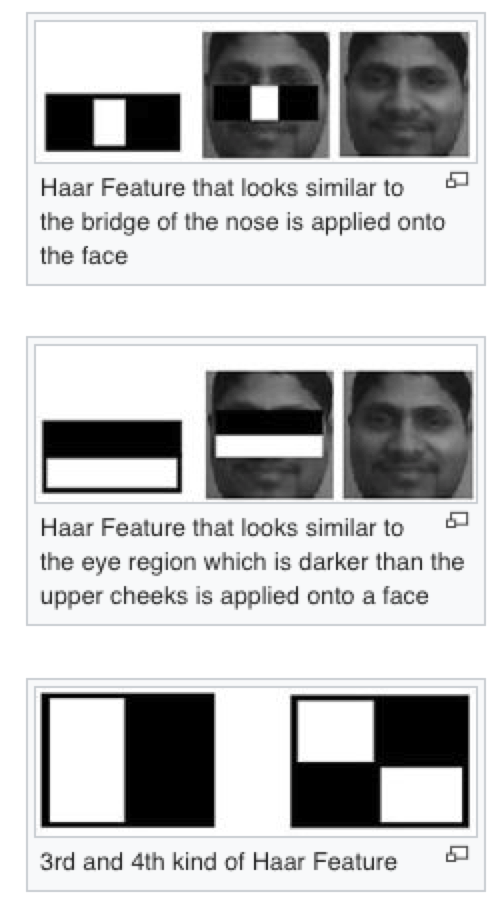
\includegraphics[scale=0.5]{./image/Haar_Feature.png}}
  \caption{Haar feature \cite{b1}.}
  \label{fig}
\end{figure}

\subsubsection{Integral Image}
Rectangle features can be computed very rapidly using an intermediate representation for the image which we call the integral image. The integral image at location x,y contains the sum of the pixels above and to the left of x,y, inclusive \cite{b2}:

\begin{equation}
 I(x,y) = \sum_{x'\leq x,y'\leq y}^{}i(x',y')
\end{equation}

In this equation, I(x,y) is the integral image, and i(x', y') is the original image, the value at any point (x, y) in the integral image is the sum of all the pixels above and to the left of (x', y') in the original image:

\begin{equation}
  I(x,y)=i(x,y)+I(x,y-1)+I(x-1,y)-I(x-1,y-1)
\end{equation}

\begin{figure}[htbp]
  \centerline{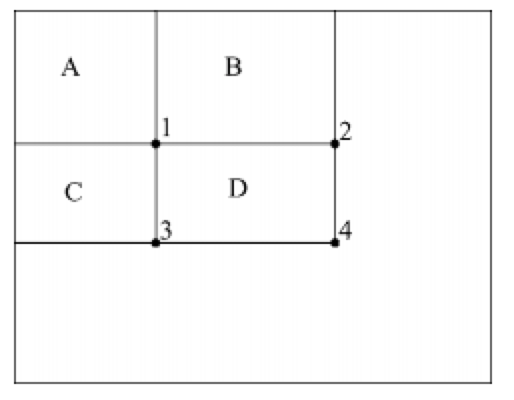
\includegraphics[scale=0.5]{./image/Integral_Image.png}}
  \caption{Integral image example.}
  \label{fig}
\end{figure}

As the example in the Fig.2, the sum of the pixels within rectangle D can be computed with four array references. The value of the integral image at location 1 is the sum of the pixels in rectangle A. The value at 2 is A + B, 3 is A + C, and at location 4 is A + B + C + D. The sum within D can be computed as 4 + 1 - 2 - 3 \cite{b2}.

\subsection{Learning Classfication Function: AdaBoost Training}
Although with the integral image, the speed is faster, but still can not adequately compensate for their number. For example, a 24x24 pixel detector, the exhaustive set of rectangle features is quite large, 160,000 \cite{b2}, and it would be prohibitively expensive to evaluate them all when testing an image. Thus, Viola-Jones Haar Algorithm employs a variant of the learning algorithm AdaBoost to both select the best features and to train classifiers that use them. This algorithm constructs a "strong" classifier as a linear combination of weighted simple "weak" classifiers.

\subsubsection{Weak Classifier To Optimal Weak Classifier}
A weak classifier $(h(x, f, p, \theta))$ consists of a sub-window image $(x)$, a feature $(f)$, a threshold $(\theta)$ and a polarity $(p)$ indicating the direction of the inequality \cite{b2}:

\begin{equation}
  h(x, f, p, \theta)= \begin{cases}
    1, & \text{if } pf(x)<p\theta\\
    0, & \text{otherwise}
  \end{cases}
\end{equation}

The $(\theta)$ is used to judge the results in comparing the feature values of the input images with the features in the weak classifier, When the value is greater than the threshold, it is determined to be a human face. The process of training the optimal weak classifier is actually looking for a suitable classifier threshold, so that the classifier has the lowest interpretation error for all samples.

\subsubsection{Strong Classifier}
Since the optimal weak classifier has been trained, the strong classifier is combined with many optimal weak classifier with some iteration.

A simplified version of the learning algorithm is reported in Algorithm 1\cite{b3}.

\begin{algorithm}
  \caption{Learning algorithm}
  \begin{algorithmic}[1]
    \renewcommand{\algorithmicrequire}{\textbf{Input:}}
    \REQUIRE Set of $N$ positive and negative training images with their labels $(x^i, y^i)$. If image $i$ is a face, then $y^i=1$, if not, $y^i=-1$
    \STATE Initialization: assign a weight $w^{i}_{1}=\frac{1}{N}$ to each image $i$.
    \FOR {each feature $f_{j}$ with $j=1,...,M$}
    \STATE Renormalize the weights such that they sum to one.
    \STATE Apply the feature to each image in the training set, then find the optimal threshold and polarity $\theta_{j}$,$s_{j}$ that minimizes the weighted classification error. That is $\theta_{j}$,$s_{j}=arg min_{\theta,s}\sum\limits^{N}_{i=1}w^{i}_{j}\varepsilon^{i}_{j}$ where $\varepsilon^{i}_{j}=\begin{cases}
      0, & \text{if } y^{i} = h_{j}(x^{i},\theta_{j},s_{j}) \\
      1, & otherwise
      \end{cases}$
    \STATE Assign a weight $\alpha_{j}$ to $h_{j}$ that is inversely proportional to the error rate. In this way best classifier are considered more.
    \STATE The weights for the next iteration, i.e. $w^{i}_{j+1}$, are reduced for the images $i$ that were correctly classified.
    \ENDFOR
    \STATE Set the final classifier to $h(x)=sgn\left(\sum\limits^{M}_{j=1}\alpha_{j}h_{j}(x) \right)$
  \end{algorithmic}
\end{algorithm}

As Algorithm 1 shown, with the iteration of M rounds, the strong classifier is then been generated with M optimal weak classifiers.

Above all, the learning process using AdaBoost is to find a threshold $\theta$ to get an optimal weak classifier from a normal weak classifier, and then generate a strong classifier with some optimal weak classifiers after some rounds iteration.

\subsection{Cascade Of Strong Classifiers}
In the Haar Detector, there are two systems, one is the training system which generates the strong classifier, since with only one strong classifier, the detector cannot guarantee the high accuracy of the detection, a good Haar Detector requires a cascade of many strong classifiers.

The other system is called detecting system, which is the process of detecting the faces in the input images with cascade detector. Since there will be plenty of sub-window images, a good cascade is strongly required to speed the detection.

The stategy of cascading strong classifiers is to arrange several strong classifiers from simple to complex. It is hoped that each strong classifier will be trained to have a high correct detection rate with low failure rate. For example, almost 99\% faces can pass one particular classifier, and 50 \% of non-human faces can also pass, so if there are 20 strong classifiers cascaded, their total correct detection rate is $0.99^{20}\approx98\%$, and the failure rate is only $0.5^{20}\approx0.0001\%$. This result can meet the needs of reality.

Strong classifiers trained by AdaBoost generally have a small false positive rate, but the correct detection rate is not very high. In general, high correct detection rate brings high false positive rate, it is caused by the threshold in the strong classifier. Increasing the correct detection rate means lower the threshold, and decreasing the false positive rate means raise the threshold, it is contradictory. According to the Viola-Jones' experiment, the increase of the classifier number can improve the detection rate of strong classifiers while reducing the false positive rate. Therefore, the cascade classifier should consider the balance during the training: 1. The balance between the number of weak classifiers and the calculation time. 2.The balance between the correct detection rate and false positive rate in strong classifiers.

A simple framework for cascade training is given below \cite{b1}:
\begin{itemize}
  \item f = the maximum acceptable false positive rate per layer.
  \item d = the minimum acceptable detection rate per layer.
  \item Ftarget = target overall false positive rate.
  \item P = set of positive examples.
  \item N = set of negative examples.
\end{itemize}

\begin{algorithm}
  \caption{The training algorithm for building a cascaded detector}
  \begin{algorithmic}[2]
    \STATE F(0) = 1.0; D(0)= 1.0; i = 0
    \WHILE {F(i) $>$ Ftarget}
      \STATE increase i
      \STATW n(i) = 0; F(i) = F(i-1)
      \WHILE {F(i) $>$ f * F(i-1)}
        \STATE increase n(i)
        \STATE use P and N to train a classifier with n(I) features using AdaBoost
        \STATE Evaluate current cascaded classifier on validation set to determine F(i) and D(i)
        \STATE decrease threshold for the ith classifier
        \STATE until the current cascaded classifier has a detection rate of at least d * D(i-1) (this also affects F(i))
        \STATE N = $\phi$
        \IF {F(i) $>$ Ftarget}
          \STATE evaluate the current cascaded detector on the set of non-face images
          \STATE and put any false detection into the set N
        \ENDIF
      \ENDWHILE
    \ENDWHILE
  \end{algorithmic}
\end{algorithm}

\section{Experiment: Camouflage Techniques}
In this coursework, I will explore how to trick the face detector through my camouflage with photographs of myself and run through the face detector to see whether the face can still be detected.

I will test all the camouflage under a range of different poses, since this detector uses only Viola-Jones algorithm which uses two rectangle features, the detector will only work for upright, near-frontal faces rather than oblique faces. (Lienhart uses oblique features to detect oblique faces)

Since the Viola-Jones Haar Cascade Algorithm uses two kinds of features which are dark-white-dark rectangle from left to right and dark-white rectangle from upper to lower, which means the forehead region, the eyes region and the nose bridge region are the key features, so I will mostly camouflage according to these features by using face paint and disguises.

\subsection{Transformation}
Since this detector uses Viola-Jones Haar features rather than using the features that Lienhart claimed in 2002 \cite{b5}, which leads that the detector can only work for upright, near-frontal faces, so transformation on the faces can also subvert the face detection.

\begin{figure}
  \centerline{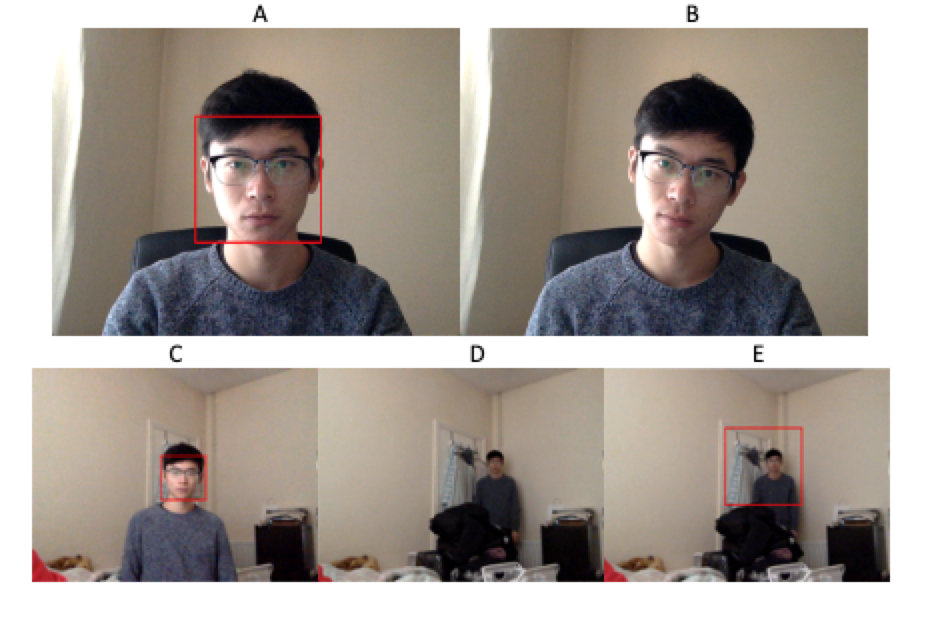
\includegraphics[scale=0.5]{./image/Transformation.png}}
  \caption{Transformation camouflage.}
  \label{fig}
\end{figure}

As shown in Fig. 3, (A) is original image which detector can detect the face. In (B), I tilted my head a little bit, and the detector can not find my face. In (C)-(E), I test the effect of distance to the detector and as shown in Fig. 3, as the distance increases, the detection effect becomes worse, it is because the base resolution of the detector is 24 x 24, which means if you stand far enough, and the face is not clear (resolution below 24 x 24), the detector can not detect it.

\subsection{Face-Paint And Make-up}
Avoid using enhancers cause they amplify key facial features which makes face easier to detect. Instead, apply makeup that contrasts with skin tone in unusual tones and directions such as, light colors to dark skin, dark colors to light skin.

The area of nose, eyes and forehead intersect is a key facial feature. Besides, the position and darkness of eyes is also a key feature. The impact of each region can be seen through the comparative images in Fig. 4.

\begin{figure}
  \centerline{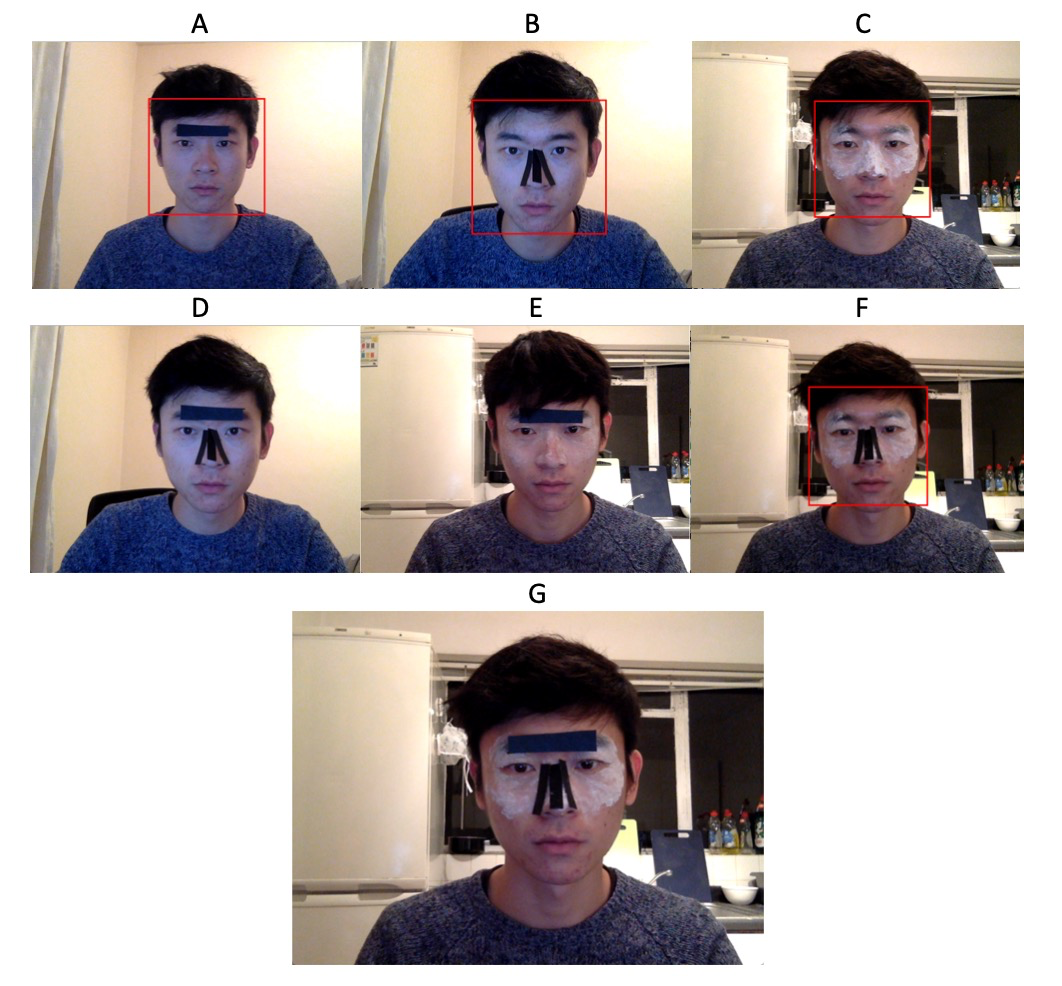
\includegraphics[scale=0.5]{./image/Face_Paint.png}}
  \caption{Face-Paint camouflage using black papers and starch. }
  \label{fig}
\end{figure}

As shown in Fig. 4, there are three rows, the first row with images (A), (B) and (C) are with only one variable which are forehead black paper in (A), nose black paper in (B) and starch on the region of eyes in (C). The second row with images (D), (E) and (F) are with two variables which are forehead black paper and nose black paper in (D), forehead black paper and starch on the region of eyes in (E), and nose black paper and starch on the region of eyes in (F). The third row with only one image (G) contains all the variables.

The results can be seen clearly, only (D), (E) and (G) subvert the face detection, though there are still many other influencing factors such as lights, hair, size of paper, facial expressions, etc., in the experiment I find that the camouflage of the forehead is the most effective one. Sometimes with only forehead black paper, the detector can not find my face.

\subsection{Disguise}
Instead of concealing the face, modify the contrast, tonal gradients, and spatial relationship of dark and light areas using hair, mask, hat or glasses, but only those can influence the key facial features are useful.

Besides, obscuring the elliptical shape of a head can also block face detection.

\begin{figure}
  \centerline{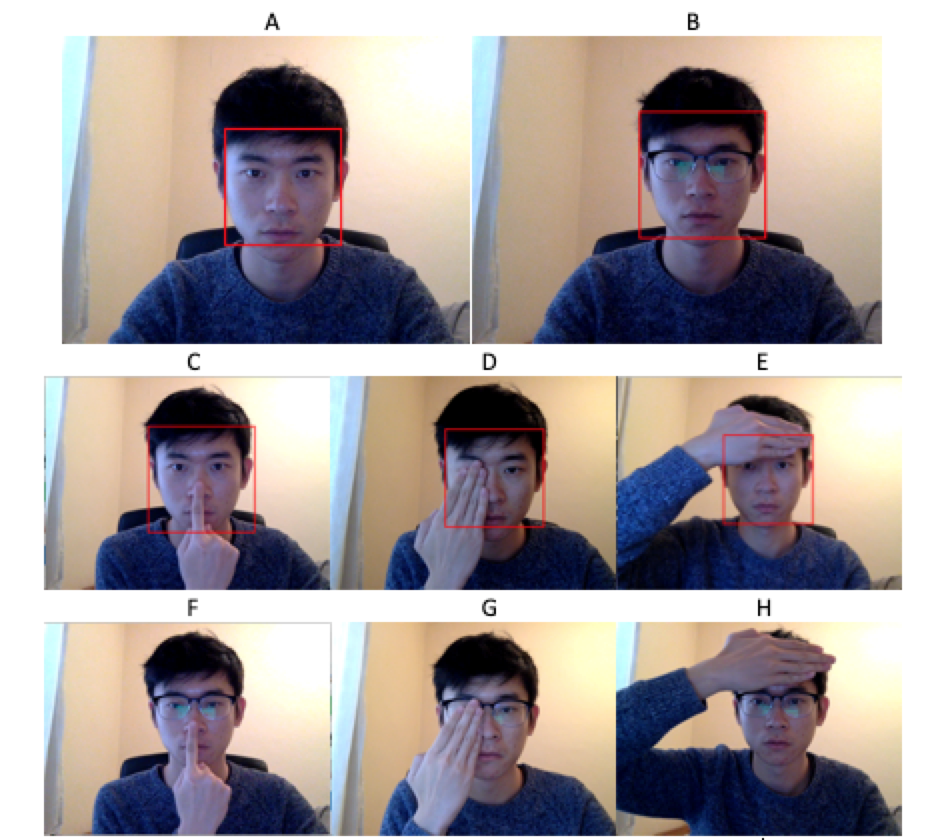
\includegraphics[scale=0.5]{./image/Disguise.png}}
  \caption{Disguise camouflage using glasses and obstruction. }
  \label{fig}
\end{figure}

As shown in Fig. 5, there are three rows, the first row with images (A), (B) show the difference between without glasses and with glasses, it is clear that with only glasses, the detector can still detects the face. In the second and third row with images (C)-(H), these images show the differences between without glasses and with glasses when I have obstructions on my face. It can be seen that the detector failed to detect the faces in (F)-(H). All the results show that glasses can subvert the face detectors only if with some obstructions.

\begin{figure}
  \centerline{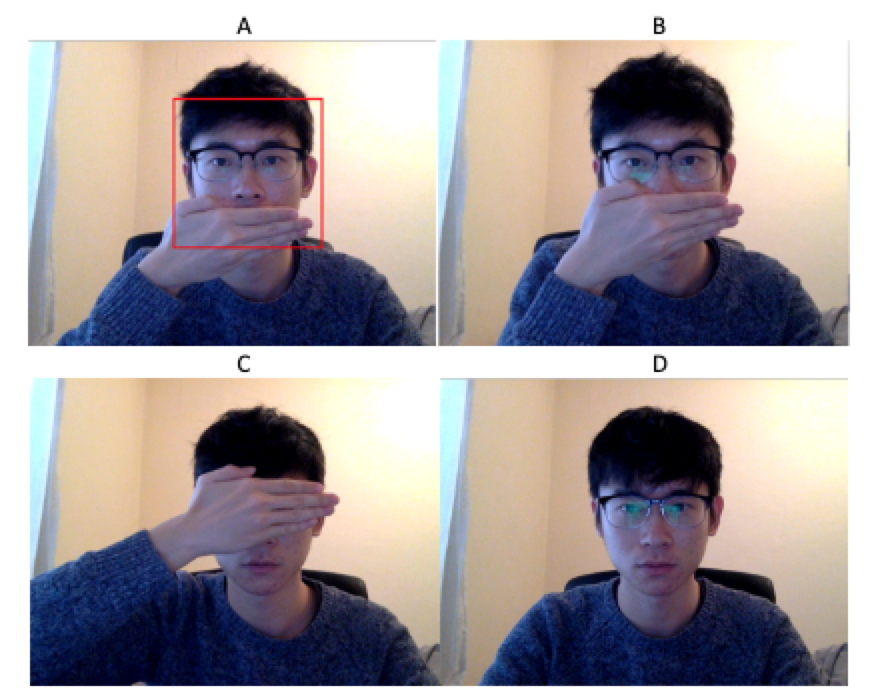
\includegraphics[scale=0.5]{./image/Disguise2.png}}
  \caption{Disguise camouflage using different obstruction positions. }
  \label{fig}
\end{figure}

As shown in Fig. 5, I experimented the effects of different positions of obstructions. It is clear that the mouth does not affect the detection, and if the face is obstructed too much, the detection is failed. Besides, I put down some hair in (D), but the detection failed too, I think it is because the hair influence the forehead region.

\section{Conclusion}
Above all, according to all the theories in the Viola-Jones Haar Algorithm and the experiments with the detectors, there are three main key features which are used to detect the faces, those features are nose bridge region, the region of eyes and the forehead region. Though there are still many other influencing factors I did not consider such as lights, sitting positions, the shape of head, the detector works mainly based on the features mentioned above.

In this coursework, I have also learned much about the face detection using the Viola-Jones Haar Cascade Algorithm. Though in this kind of algorithm, only two simple features are used, the detector's effect is still good, if use features that Lienhart claimed \cite{b5}, the correct detection rate can be very high.

Besides, though Viola and Jones used AdaBoost to speed the detection, the time cost is still high. I have read many papers and find that the detection area in the sub-window images is the key point, decreasing the unnecessary detection area can significantly improve the performance. Some people use a rough estimate of the area of the skin in the image to locate the approximate face range to greatly reduce the size of the detected image. Others use the influence of each frame of the video on the next frame to constrain the search range. I think both can increase the performance and raise the correct detection rate.

\begin{thebibliography}{00}
\bibitem{b1} En.wikipedia.org. (2018). Viola–Jones object detection framework. [online].
\bibitem{b2} Viola, P. and Jones, M. (2004). ``Robust Real-Time Face Detection.`` International Journal of Computer Vision, 57(2), pp.137-154.
\bibitem{b3} R. Szeliski, Computer Vision, algorithms and applications, Springer.
\bibitem{b4} Harvey, A. (2018). ``CV Dazzle: Camouflage from Face Detection``. [online] Cvdazzle.com. Available at: https://cvdazzle.com/ [Accessed 20 Nov. 2018].
\bibitem{b5} Lienhart, R. and Maydt, J., 2002. An extended set of haar-like features for rapid object detection. In Image Processing. 2002. Proceedings. 2002 International Conference on (Vol. 1, pp. I-I). IEEE.
\end{thebibliography}

\end{document}
